\documentclass[12pt]{article}

% --- document setup and text -----------------------

% document class defines document-wide parameters. 
% You will probably use ``article'' for everything but posters and slides

\usepackage[margin = 1in]{geometry} % controls page margins
\usepackage{setspace}               % controls line spacing

\usepackage{parskip}
% ``parskip'' is used to get (a) space between paragraphs and
% (b) no indentation at new paragraphs.
% This makes this particular document easier to read, 
% but I do NOT recommend using parskip ordinarily
% (except for problem sets maybe)
                     

% --- math things -----------------------

\usepackage{amsmath} % commonly used for enhanced math commands
\usepackage{amssymb} % commonly used for helpful symbols and fonts
                     % many people also load ``amsfonts''
                     % but amssymb loads amsfonts, so it's not necessary



% --- tables, figues, other floats -----------------------

\usepackage{float}    % float parameters

% graphics:
\usepackage{graphicx} % capabilites for inserting graphics
\usepackage{rotating} % if you want sideways graphics
\usepackage{subcaption} % if you want sub-figures
% \usepackage{placeins} 
%   ``placeins'' contains a helpful \FloatBarrier command
%   which prevents figures from bleeding across sections


% tables
\usepackage{booktabs} % commonly used to make tables prettier
\usepackage{dcolumn} % aligns table column text along a decimal pt
\usepackage{multirow, multicol} % cells spanning multi rows/cols



% --- other document logic/capabilities -----------------------

\usepackage{hyperref}  % hyperlinks
\usepackage{xcolor}    % more colors (don't go too crazy)
\usepackage{todonotes} % print yourself to-do notes



% --- fancy code blocks -----------------------

% WARNING to workshop participants:
% These ``listings'' settings are included to make code blocks prettier,
% but ``listings'' is not essential unless you want to include code
% which should be rare unless you're describing computer algorithms.
% I would NOT paste these settings into your future work.

% If you're interested in printing code, you might also check out ``minted''.
% Minted prints prettier code blocks, 
% but it depends on pygments (http://pygments.org/) which can be a pain

\usepackage{listings}

\definecolor{lgray}{gray}{0.925}

\lstset{ 
  backgroundcolor = \color{lgray},
  basicstyle = \ttfamily, % code style
  breakatwhitespace = true,      % if automatic break only happen at whitespace
  breaklines = false,            % automatic line breaking
  columns=fullflexible,          % kerning thing
  commentstyle = \color{gray},   % comment style
  escapeinside = {\% *}{*)},     % for using LaTeX within code
  keepspaces = true,             % keeps spaces for indentation 
                                 % (needs columns = flexible ?)
  language = TeX,                % the language of the code
  % morekeywords = {*,...},        % for adding more keywords
  showstringspaces = false      % underline spaces within strings only
}





\begin{document}

\title{{\LaTeX} Starter Guide}
\author{Michael DeCrescenzo%
          \thanks{Ph.D.\ Candidate, Political Science, University of Wisconsin--Madison. This handout borrows heavily past workshop materials created and passed down by Matthew Holleque, Sarah Niebler, and Dave Ohls, Sarah Bouchat, Nat Olin, Richard Loeza, and Jos\'e Luis Enr\'iquez Chi\~nas, and Michael Masterson.}}
\date{Updated \today}
\maketitle


\begin{abstract}
  This document describes and exemplifies many important {\LaTeX} concepts and best-practices. It discusses document setup, important commands and environments, text formatting, math, figures and tables, and so on. This document (a \lstinline{.pdf} file) is distributed alongside the source code used to create it (a \lstinline{.tex} file), allowing new {\LaTeX} users to see how {\LaTeX} code becomes printed content. The source code, along with other workshop materials, can be found on the workshop's Github page.%
    \footnote{\url{https://github.com/mikedecr/latex-workshop-2018}}
\end{abstract}



\section{How to read this document}

This document is intended to teach {\LaTeX} by example. The text contains a discussion of {\LaTeX} commands, but for instructional purposes it will also be valuable to download, inspect, and modify the source code%
  \footnote{I advise that you preserve an original copy of the source code, for future reference. The file can be copied from here: \url{https://raw.githubusercontent.com/mikedecr/latex-workshop-2018/master/handout/latex-handout-2018.tex}} yourself. 

Examples of {\LaTeX} code will appear in the text. These examples are printed with a \lstinline{monospace} font. If we want to view a lot of code at once, we will see code presented in a code block. Code blocks are styled to make them easier to read:

\begin{lstlisting}
  This is where
  a lot
  of code
  would be written at once
\end{lstlisting}

It is important to distinguish the code that builds the document from the example code that is printed in the final document. The code that builds the document isn't directly visible to you---it is interpreted by the {\TeX} compilation engine to create the final document. The example code that appears in the final text is simply printed, not executed.%
  \footnote{We discuss how to print code without executing it later in this document.}



\section{Essentials}

{\LaTeX} works like this. 
\begin{enumerate}
  \item \textbf{Source code.} You start with a plain text file (with a \lstinline{.tex} extension), which serves as the source code for your final document. The source contains the text of your document (unstyled) and code to ``mark up'' the text. The markup code provides logical structure and stylistic guidelines for the text to follow. 
  \item \textbf{Compilation.} The source code is compiled by the {\TeX} engine. The engine interprets the markup code to learn which text serves what purpose, and it follows those instructions to build the final document. The compilation process runs into errors if the compiler can't interpret the source file.
  \item \textbf{Output.} Successful compilation returns an output document, usually a \lstinline{pdf} file (usually a \emph{pretty} \lstinline{pdf} file).
\end{enumerate}



{\LaTeX} ``source'' documents are \lstinline{.tex} files. 

They require you to declare a document class at the very top of the file. The most common class is \texttt{article}, but other options include \texttt{paper}, \texttt{book}, \texttt{memoir}, \texttt{report}, and so on. Details about these other classes can be found online.

The content of the document lies in the \texttt{document} environment. Environments are delineated with \verb+\begin{environment}+ and \verb+\end{environment}+ tags.

The most basic document you could create, therefore, would look like the following:

\begin{minipage}{\linewidth}
\begin{lstlisting}
  \documentclass{article} 

  \begin{document} 
    Hello, world! 
  \end{document}
\end{lstlisting}
\end{minipage}

  {\LaTeX} contains a number of additional functionalities, but not all are loaded by default. You can load packages for {\LaTeX} capabilities using the \verb+\usepackage{package-name}+ command. You would place package-loading commands in the \emph{preamble}, which is the part of the \texttt{.tex} document between the \verb+\documentclass+ and the \texttt{document} environment.

  Some packages allow you to tweak additional settings with further commands. These commands must be included \emph{after} the \verb+\usepackage+ command.


\section{Titles and Abstracts}

  Creating titles in {\LaTeX} is easy.

  \begin{verbatim}
    \title{Title here}
    \author{Author name here}
    \date{Type a date or use the \today command}
    \maketitle
  \end{verbatim}

  {\LaTeX} will take care of the formatting, so you don't have to waste your time with it.

  For articles and conference papers, you can also include abstracts.

  \begin{verbatim}
  \begin{abstract}
    Here's what this paper is going to be about.
  \end{abstract}
  \end{verbatim}



\section{Chapters, Sections, Subsections, \dots}

  It is common to organize a document with sections. Available section levels are \texttt{section}, \texttt{subsection}, and \texttt{subsubsection}. 

  \begin{verbatim}
  \section{Section}
  \subsection{Subsection}
  \subsubsection{Subsubsection}
  \end{verbatim}

  If you put a * after the section command, it will suppress section numbering.

  \begin{verbatim}
  \subsection{Subsection with a number}
  \subsection*{Subsection without a number}
  \end{verbatim}

  The above commands would create the following subsection titles:

  \subsection{Subsection with a number}
  \subsection*{Subsection without a number}


  The \texttt{book} and \texttt{report} classes also allow you to use \verb+\part+ and \verb+chapter+ structures.



\section{Aligning Left, Right, and Center}

  You can align your your document using different alignment environments.
  \begin{flushleft}
  You can align text to the left with the \texttt{flushleft} environment.
  \end{flushleft}

  \begin{flushright}
  You can align text to the right with the \texttt{flushright} environment.
  \end{flushright}

  \begin{center}
  You can align text to the center with the \texttt{center} environment.
  \end{center}


\section{Spacing}

  \subsection*{Line Spacing}
  
  You can use the \texttt{setspace} package to allow for double spacing (and other space factors). Just add \verb+\usepackage{setspace}+ to the preamble, and add \verb+\doublespacing+ to the body of the document. The \texttt{setspace} package also allows \verb+\singlespacing+, \verb+\onehalfspacing+ for 1.5 spacing, and custom spaces using \verb+\setstretch{x}+. These commands also have environment versions, in case you want to take finer control of the document. 
  \begin{verbatim}
  \begin{singlespace}
    This text would be single spaced.
  \end{singlespace}

  \begin{doublespace}
    This text would be double spaced.
  \end{doublespace}
  \end{verbatim}

  \subsection*{Vertical Space}
  You can use the \verb+\vspace{}+ command to insert blank space.  You put an amount of space inside the \verb+{}+. Let's say you wanted to leave a one-inch space before the next line. \verb+\vspace{1in}+ would do it.

  \vspace{1in}

  Check it out.

  While taking fine control of vertical space within a document is \emph{possible}, it is generally against the {\LaTeX} philosophy to take such fine control. It is smarter to set your desired global options in the document's preamble, leaving the document body itself free of tedious stylistic manipulation.




\subsection{Line Breaks, Page Breaks, and Blank Pages}

There are several ways to to create a new paragraphs and line breaks.

New paragraphs are created by leaving a blank line between two blocks of text in your \texttt{.tex} file.

You can also force a single line break by typing \verb+\\+ or \verb+\newline+ at the end of a line. New lines are not the same as paragraph breaks; indentation rules will apply to new paragraphs but not new lines.

To insert a page break, you can use either the \verb+\newpage+ or \verb+\clearpage+ commands.

\clearpage


\section{Indentation}

{\LaTeX} will automatically indent new paragraphs, but you can stop that behavior by adding \verb+\noindent+ before a new paragraph. 

A document's overall indentation behavior is something you want to set with global parameters in the preamble rather than with \verb+\noindent+ commands throughout your entire document. For example, this document uses \verb+\usepackage{parskip}+ to (a) add space between paragraphs and (b) prevent indentation in new paragraphs. These \texttt{parskip} package defaults can be overridden if you include more commands in the preamble after loading the package (see package documentation).


\section{Commenting}

  You can use the \% to write comments in the code. This way, you can leave notes that don't show up in the document.

  \begin{verbatim}
    % This would not show up in a normal document.
  \end{verbatim}

  The \texttt{comment} package provides a comment environment.
  \begin{verbatim}
    \begin{comment}
      You can write 

      long

      comments

      that span multiple paragraphs

      and none of the text would show up in the final document.
    \end{comment}
  \end{verbatim}
  I have found the \texttt{comment} package to be quite handy when writing  and revising papers. 

  Bonus: the \texttt{todonotes} package also provides cool way to leave notes to yourself in a document using \verb+\todo{}+. \todo{Useful} You can modify the appearance of the bubbles in the package options.
  


\section{Font Sizes}

  Font sizes can be done with inline commands or in environments. The sizes (and size ``names'' are\dots

  \begin{tiny}tiny\end{tiny}
  \begin{scriptsize}scriptsize\end{scriptsize}
  \begin{footnotesize}footnotesize\end{footnotesize}
  \begin{small}small\end{small}
  \begin{normalsize}normalsize\end{normalsize}
  \begin{large}large\end{large}
  \begin{Large}Large\end{Large}
  \begin{LARGE}LARGE\end{LARGE}
  \begin{huge}huge\end{huge}
  \begin{Huge}Huge\end{Huge}

  Inline sizing can be done {\huge like so}.

  \begin{verbatim}
    Inline sizing can be done {\huge like so}.
  \end{verbatim}

  \begin{tiny}
    Or you can use an environment.
  \end{tiny}

  \begin{verbatim}
  \begin{tiny}
    Or you can use an environment.
  \end{tiny}
  \end{verbatim}



\section{Font Styles}

  Inline font styling (emphasis, bolding) is handled with inline commands as well. Emphasizing is handled with \verb+\emph{}+, bolding with \verb+\textbf{}+.

  Although most typefaces and document classes don't show the difference, \textit{italicizing} and \emph{emphasizing} can sometimes look different. \textsl{Slanting} (\verb+textsl{}+) is also different from \textit{italicizing}, so that is another distinction to keep in mind.

  You can write fixed-width font using the ``teletype'' font, accomplished using \verb+\texttt{}+. \texttt{This is teletype.}

  \textsc{Small Capitals} can be accomplished with \verb+\textsc{}+.


\section{Verbatim}

  You can use the \texttt{verbatim} environment to print text \emph{exactly} how it appears. This is useful for writing {\LaTeX} commands without executing them. It can also be a nice way to display output from other programs (like R).

  \begin{verbatim}
  This text here created inside the verbatim environment.
  \end{verbatim}

  You can do  \verb+inline verbatim+ as well.

  \begin{verbatim}
    You can do  \verb+inline verbatim+ as well.
  \end{verbatim}



\section{Special Characters}

  Certain characters have special meaning in {\LaTeX}. In order to use them, you have to include escape characters (a backslash) or type a special command.

  \# \$ \% \& \_ \{\} $\tilde{}$ $\grave{}$ \textbackslash

  \begin{verbatim}
  \# \$ \% \& \_ \{\} $\tilde{}$ $\grave{}$ \textbackslash
  \end{verbatim}

  \$300 is 50\% of my take-home pay.

  \begin{verbatim}
  \$300 is 50\% of my take-home pay.
  \end{verbatim}

  Some of these special characters affect the characters immediately after them. For example, my old roommate (Jos\'e Luis Enr\'iquez Chi\~nas) must have a difficult type {\TeX}ing his name:
  \begin{verbatim}
  Jos\'e Luis Enr\'iquez Chi\~nas
  \end{verbatim}

\section{Quotation Marks}

  Quotes are a little funky in {\LaTeX} because it takes the direction of the quote mark literally. To get normal looking quotation marks, use the accent key for opening quotes and apostrophes or double quotes for closing quotes.

  "Political Science is fun!" Looks wrong.

  ``Political Science is fun!''  Looks much better.

  \begin{verbatim}
  "Political Science is fun!" Looks wrong.

  ``Political Science is fun!''  Looks much better.
  \end{verbatim}


\section{Dashes}

  Your professors care about the following distinctions. They are also important to get right using {\LaTeX}.

  One dash \verb+-+ is a hyphen. Example: cold-blooded (\verb+cold-blooded+).

  Two dashes \verb+--+ is an en-dash. Example: University of Wisconsin--Madison \\ (\verb+University of Wisconsin--Madison+)

  Three dashes \verb+---+ is an em-dash. Example: Nietzsche---who greatly overueses em-dashes---once wrote\dots  \\
  (\verb+Nietzsche---who greatly overueses em-dashes---once wrote\dots+)



\section{Footnotes}

  To enter text in a footnote, type \verb+\footnote{}+ and include whatever text you want in the brackets.\footnote{Very exciting footnote text.} Footnotes go \emph{after} punctuation, in case you were wondering.


\section{Lists}

  {\LaTeX} has separate \texttt{itemize} and \texttt{enumerate} for creating unordered and ordered lists, respectively.

  An unordered list:

  \begin{itemize}
    \item{First item on the list}
    \begin{itemize}
      \item{First item on the sublist}
      \item{Second item on the sublist}
    \end{itemize}
    \item{Second item on the list}
  \end{itemize}

\begin{verbatim}
An unordered list:

\begin{itemize}
  \item{First item on the list}
  \begin{itemize}
    \item{First item on the sublist}
    \item{Second item on the sublist}
  \end{itemize}
  \item{Second item on the list}
\end{itemize}
\end{verbatim}

An ordered list: 

\begin{enumerate}
  \item{First item on the list}
  \begin{enumerate}
    \item{First item on the sublist}
    \item{Second item on the sublist}
  \end{enumerate}
  \item{Second item on the list}
\end{enumerate}

\begin{verbatim}
An ordered list: 

\begin{enumerate}
  \item{First item on the list}
  \begin{enumerate}
    \item{First item on the sublist}
    \item{Second item on the sublist}
  \end{enumerate}
  \item{Second item on the list}
\end{enumerate}
\end{verbatim}

You could customize the character beside a list item with square brackets after \verb+\item+. For example, \verb+\item[/] Item text+ would create list items like
\begin{itemize}
  \item[/] Item text
\end{itemize}
\dots although as with many things in {\LaTeX}, it's efficient for you \emph{note} to sweat the small stuff like this. 




\section{Math Basics}

  One of the most attractive and powerful features of {\LaTeX} is its ability to typeset complex mathematical notation via ``math mode''. Math mode can be invoked inline by wrapping an expression in dollar signs (\$). For example, \verb+$e=mc^2$+, is rendered as $e=mc^2$. Alternatively, a variety of commands allow you set equations apart from the main body of your text. For example:

  \begin{quote}\begin{verbatim}
  \begin{equation}
  y = \beta_1 + \alpha
  \end{equation}
  \end{verbatim}\end{quote}
  Renders as: 
  \begin{equation}
  y = \beta_1 + \alpha
  \end{equation}

  If you would like to suppress the equation numbering, you can add an asterisk to the end of the command (\verb+\begin{equation*}...\end{equation*}+). One nice shorthand: \verb+\[...\]+ is equivalent to \verb+\begin{equation*}...\end{equation*}+.


\subsection{Fractions}
  
  To write fractions, simply use \verb+\frac{}{}+ and place the numerator of the fraction in the first set of brackets and the denominator of the fraction in the second set of brackets. You can also embed fractions within fractions. For example, $\frac{1}{2}$ or $\sum\frac{x_{i}-\bar{x}}{n-1}$. Producing these fractions is straight forward, but sometimes the nested code blocks can be difficult to read.: 
  \begin{quote}\begin{verbatim}
  $\frac{1}{2}$
  $\sum\frac{x_{i}-\bar{x}}{n-1}$
  \end{verbatim}\end{quote}


\subsection{Greek Letters}
  
  To write Greek letters, simply write a backslash and the name of the letter after the slash. For example, \verb+$\beta$+ and \verb+$\sigma$+ renders as $\beta$ and $\sigma$. Note that capitalizing the first letter of the Greek letter name gives you a capital Greek letter. So, \verb+$\Delta$+ renders as $\Delta$, but \verb+\delta+ is $\delta$. For some Greek letters, such alpha, the capital is the same as the Roman. In cases like these, you just use the Roman---there is no \verb+$\Alpha$+, only $A$.

  When there are multiple versions of the same Greek letter, you can use the \verb+var+ prefix to use the alternate. For example, \verb+$\epsilon = \varepsilon$+ will render as $\epsilon = \varepsilon$. 

  A complete list of commands for the Greek alphabet is available at \url{http://jblevins.org/notes/greek}.

\subsection{Operators and Other Symbols}

  Numerous symbols can be used in the math environment. Commonly used symbols include inequalities, set notation, and operators. Many of these are straight forward (e.g. equals, greater than, less than), but many are not. We review a few commonly used symbols and operators below. 

  To write a summation sign or a product sign, the commands are \verb+\sum and \prod+, which produce $\sum$ and $\prod$ respectively. 

  For inequalities, the commands are \verb+\neq+, \verb+\ge+, \verb+\le+, and these produce $\neq$, $\ge$, and $\le$ respectively. 

  Common set notation commands include \verb+\mathbb{R}+ ($\mathbb{R}$), \verb+\in+ ($\in$), \verb+\not \in+ ($\not \in$), \verb+\mid+ ($\mid$). Because curly braces are interpreted by the {\LaTeX} compiler, you need to escape them with a backslash whenever you use them in math mode. So, \verb+{...}+ will either not render or cause an error. Instead, use \verb+\{...\}+. This will render as $\{...\}$. Putting it all together, we can write \verb+$\mathbb{A} \in \{1,2,3\}$+, which will render as $\mathbb{A} \in \{1,2,3\}$.

  You may also want to be aware that operators and functions like $\max_{x_L}$, $\ln (x)$, $\lim\limits_{x \to +\infty}$, $\int$, and $\partial$ are also {\LaTeX} commands. You can read more about these and other commands here: \url{http://en.wikibooks.org/wiki/LaTeX/Mathematics}.

\subsection{Hats and Bars}

  To place a hat or a bar over any math character, simply place the text in brackets after the writing \verb+\bar{}+ or \verb+\hat{}+ commands. \verb+$\bar{\beta} \neq \hat{y}$+ gives us $\bar{\beta} \neq \hat{y}$.


\subsection{Superscripts and Subscripts}

  To write a superscript, write \verb+^{}+ with the text of the superscript in the brackets. If you just have one character in the superscript, you do not have to include the brackets. For example, \verb+$x^3$+ renders as $x^3$ or \verb+$e^{-z\gamma}$+ renders as $e^{-z\gamma}$.

  If you forget the brackets, as in \verb+$e^-z\gamma$+, the superscript will render as $e^-z\gamma$. (I wrote my own keyboard shortcuts for Sublime Text to always insert curly brackets after a \verb+^+ to prevent these kinds of mistakes.)

  To write a subscript, write \verb+_{}+ with the text of the subscript in the brackets. Again, if you have just one character in the subscript, you do not have to include the brackets. For example, \verb+$x_1$+ renders as $x_1$ and \verb+$x_{ij}$+ renders as $x_{ij}$.

  Some commands allow you to use the subscript and superscript environments together to place notation on top of or underneath other notation. For example, \verb+$\sum_{i=0}^{100} i$+ renders as $\sum_{i=0}^{100} i$. 

  To make it look a little better, we can add the command \verb+\limits+ after the \verb+\sum+ command: \verb+$\sum\limits_{i=0}^{100} i$+. From this we get: 

  \[
  \sum\limits_{i=0}^{100} i
  \]

  Including \verb+\displaystyle+ before the $\sum$ accomplishes a similar effect. This can also improve limit expressions ($\displaystyle\lim_{x\to\infty}$) and integrals ($\displaystyle\int^y_x$). Display style will also slightly increase the size of your expressions in in-line math, which can prevent complicated math from getting shrunk too small in the middle of a block of text.

\section{More Complicated Math}
  
  Now, for more complicated math, you can use the \texttt{align} environment, which will align a set of equations along an operator of your choice. To pick the operator on which you want to align your list of equations, place a \verb+&+ in front of it. For multiple lines, you need to place two backslashes at the end of each line of equations, and there should be no empty lines anywhere in the \verb+align+ environment. Take a look at the following, which will not compile correctly: 
  \begin{quote}\begin{verbatim}
  \begin{align}

  \ln(L) &= n \ln(\alpha) + n \ln (x) - n \ln (x)\\
  \frac{d \ln(L)}{d\alpha} &= \frac{n}{\alpha} + n \ln(x) - 0\\
  \frac{n}{\alpha} + n \ln(x) &= 0\\
  \frac{n}{\alpha} &= -n \ln(x)\\
  n &= \alpha (-n \ln(x))\\
  \alpha &= \frac{n}{-n \ln(x)}\\
  \alpha &= \frac{-1}{\ln(x)}\\
  \end{align}
  \end{verbatim}
  \end{quote}

  This, however will compile correctly: 
  \begin{quote}\begin{verbatim}
  \begin{align}
  \ln(L) &= n \ln(\alpha) + n \ln (x) - n \ln (x)\\
  \frac{d \ln(L)}{d\alpha} &= \frac{n}{\alpha} + n \ln(x) - 0\\
  \frac{n}{\alpha} + n \ln(x) &= 0\\
  \frac{n}{\alpha} &= -n \ln(x)\\
  n &= \alpha (-n \ln(x))\\
  \alpha &= \frac{n}{-n \ln(x)}\\
  \alpha &= \frac{-1}{\ln(x)}\\
  \end{align}
  \end{verbatim}
  \end{quote}

  It renders as: 
  \begin{align*}
  \ln(L) &= n \ln(\alpha) + n \ln (x) - n \ln (x)\\
  \frac{d \ln(L)}{d\alpha} &= \frac{n}{\alpha} + n \ln(x) - 0\\
  \frac{n}{\alpha} + n \ln(x) &= 0\\
  \frac{n}{\alpha} &= -n \ln(x)\\
  n &= \alpha (-n \ln(x))\\
  \alpha &= \frac{n}{-n \ln(x)}\\
  \alpha &= \frac{-1}{\ln(x)}\\
  \end{align*}

  You can add additional space (or subtract space) between lines by specifying skip lengths in square brackets. Example:
  \begin{verbatim}
  \begin{align*}
    a &= 1 \\
    a &= 1 \\[6pt]
    a &= 1 \\[12pt]
    a &= 1
  \end{align*} 
  \end{verbatim}
  \dots renders as\dots
  \begin{align*}
    a &= 1 \\
    a &= 1 \\[6pt]
    a &= 1 \\[12pt]
    a &= 1
  \end{align*}



\section{Figures}

  % primarily relying on the graphicx package

  The fundamental component of including a graphic or figure is the \verb+\includegraphics+ command.  Here, the syntax \verb+\includegraphics[width=10cm]{extensions.png}+ specifies that it should include the figure with filename \textit{extensions.png}\footnote{If the filename isn't in the same directory as the .tex file, you'll need to specify the full file path.  Generally, it's simpler to just make sure all files called are in the same folder.} with a width of 10 centimeters (it will automatically adjust the height of the figure along with this). 

  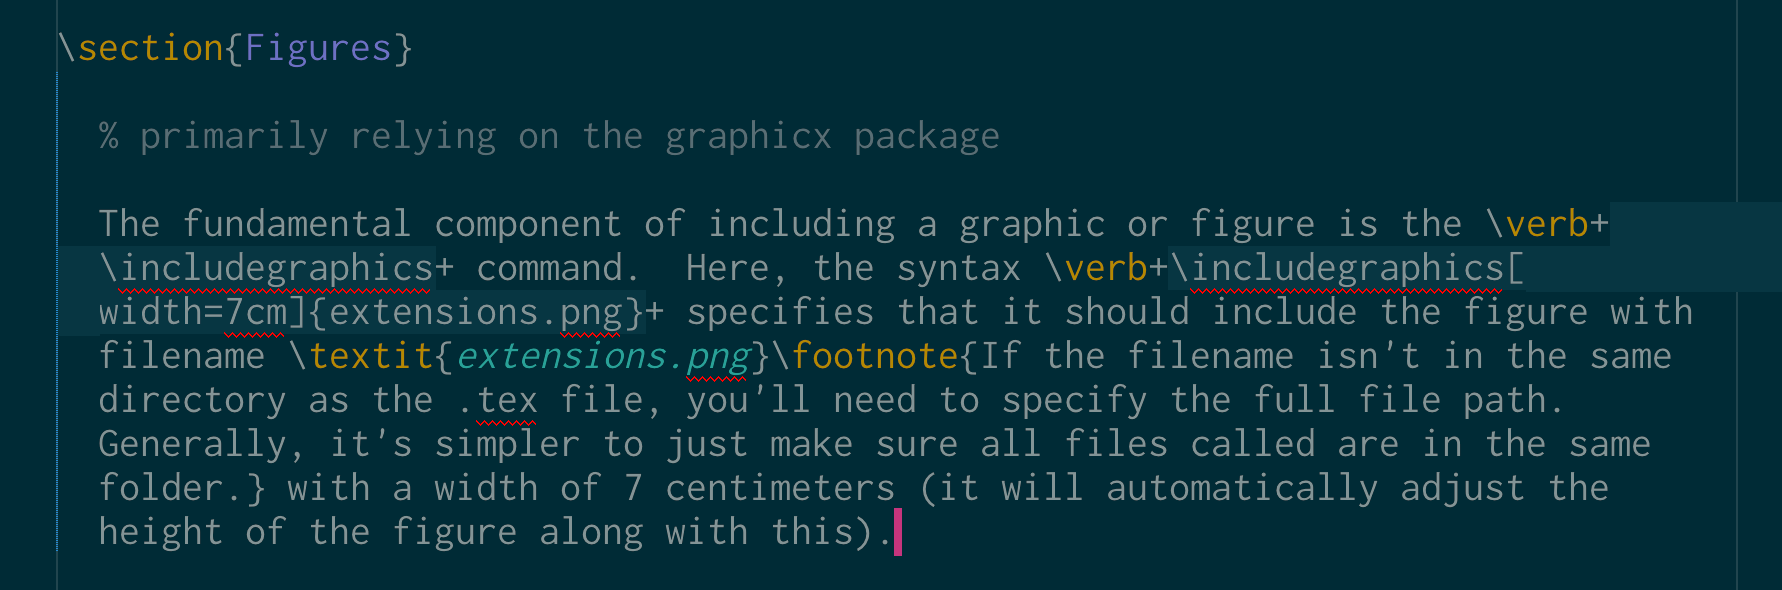
\includegraphics[width=10cm]{imgs/text-cap.png}

  To create figures with accessories, it is often useful to put it in a `float' using the \textit{figure} environment, which is generally good practice for figures.  This allows captions and other elements to be included and automatically associated with the figure.

  Sizing can be done as a fraction of the width of the text using \verb+[width = x\textwidth]+ where \texttt{x} is the proportion of the text width that the graphic fills.

  The following code inserts a graphic of Pok\'emon statistics:
  \begin{verbatim}
  \begin{figure}[!ht]
    \centering
    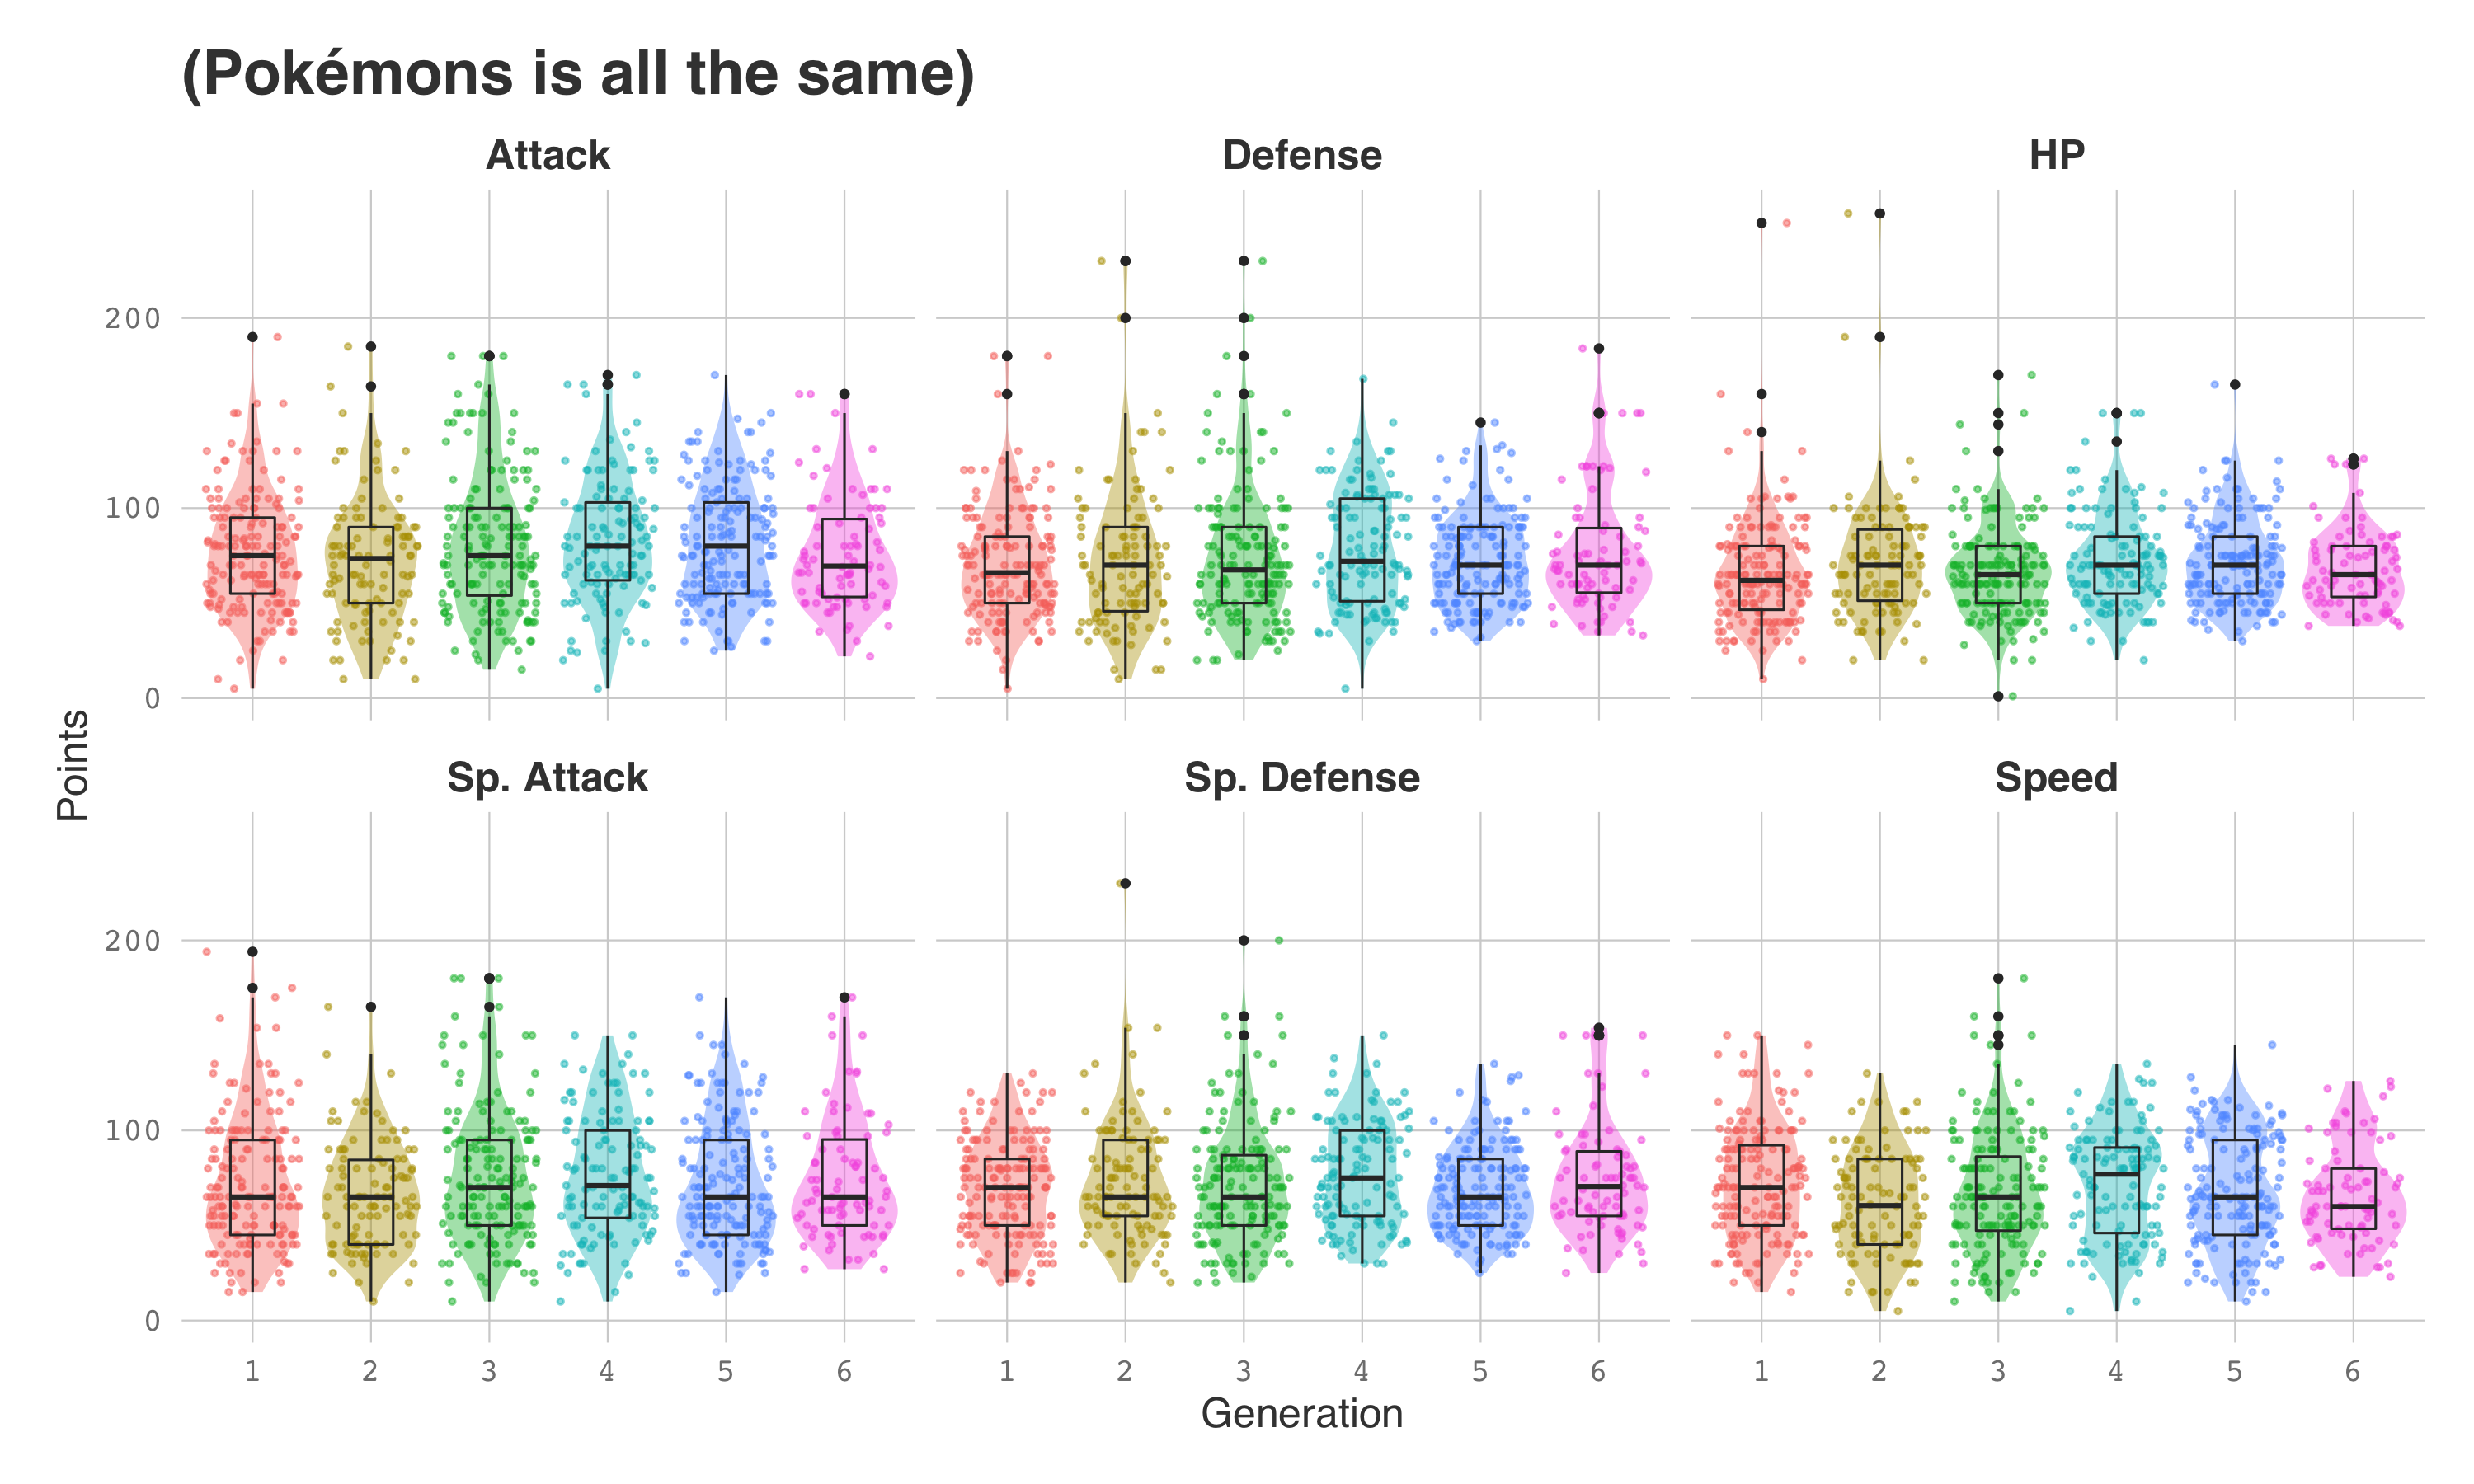
\includegraphics[width = \textwidth]{imgs/specs-gen-vio-box.png}
    \caption{Distribution of Pok\'emon Stats}
    \label{fig:poke-stats}
  \end{figure}
  \end{verbatim}

  \begin{figure}[ht]
    \centering
    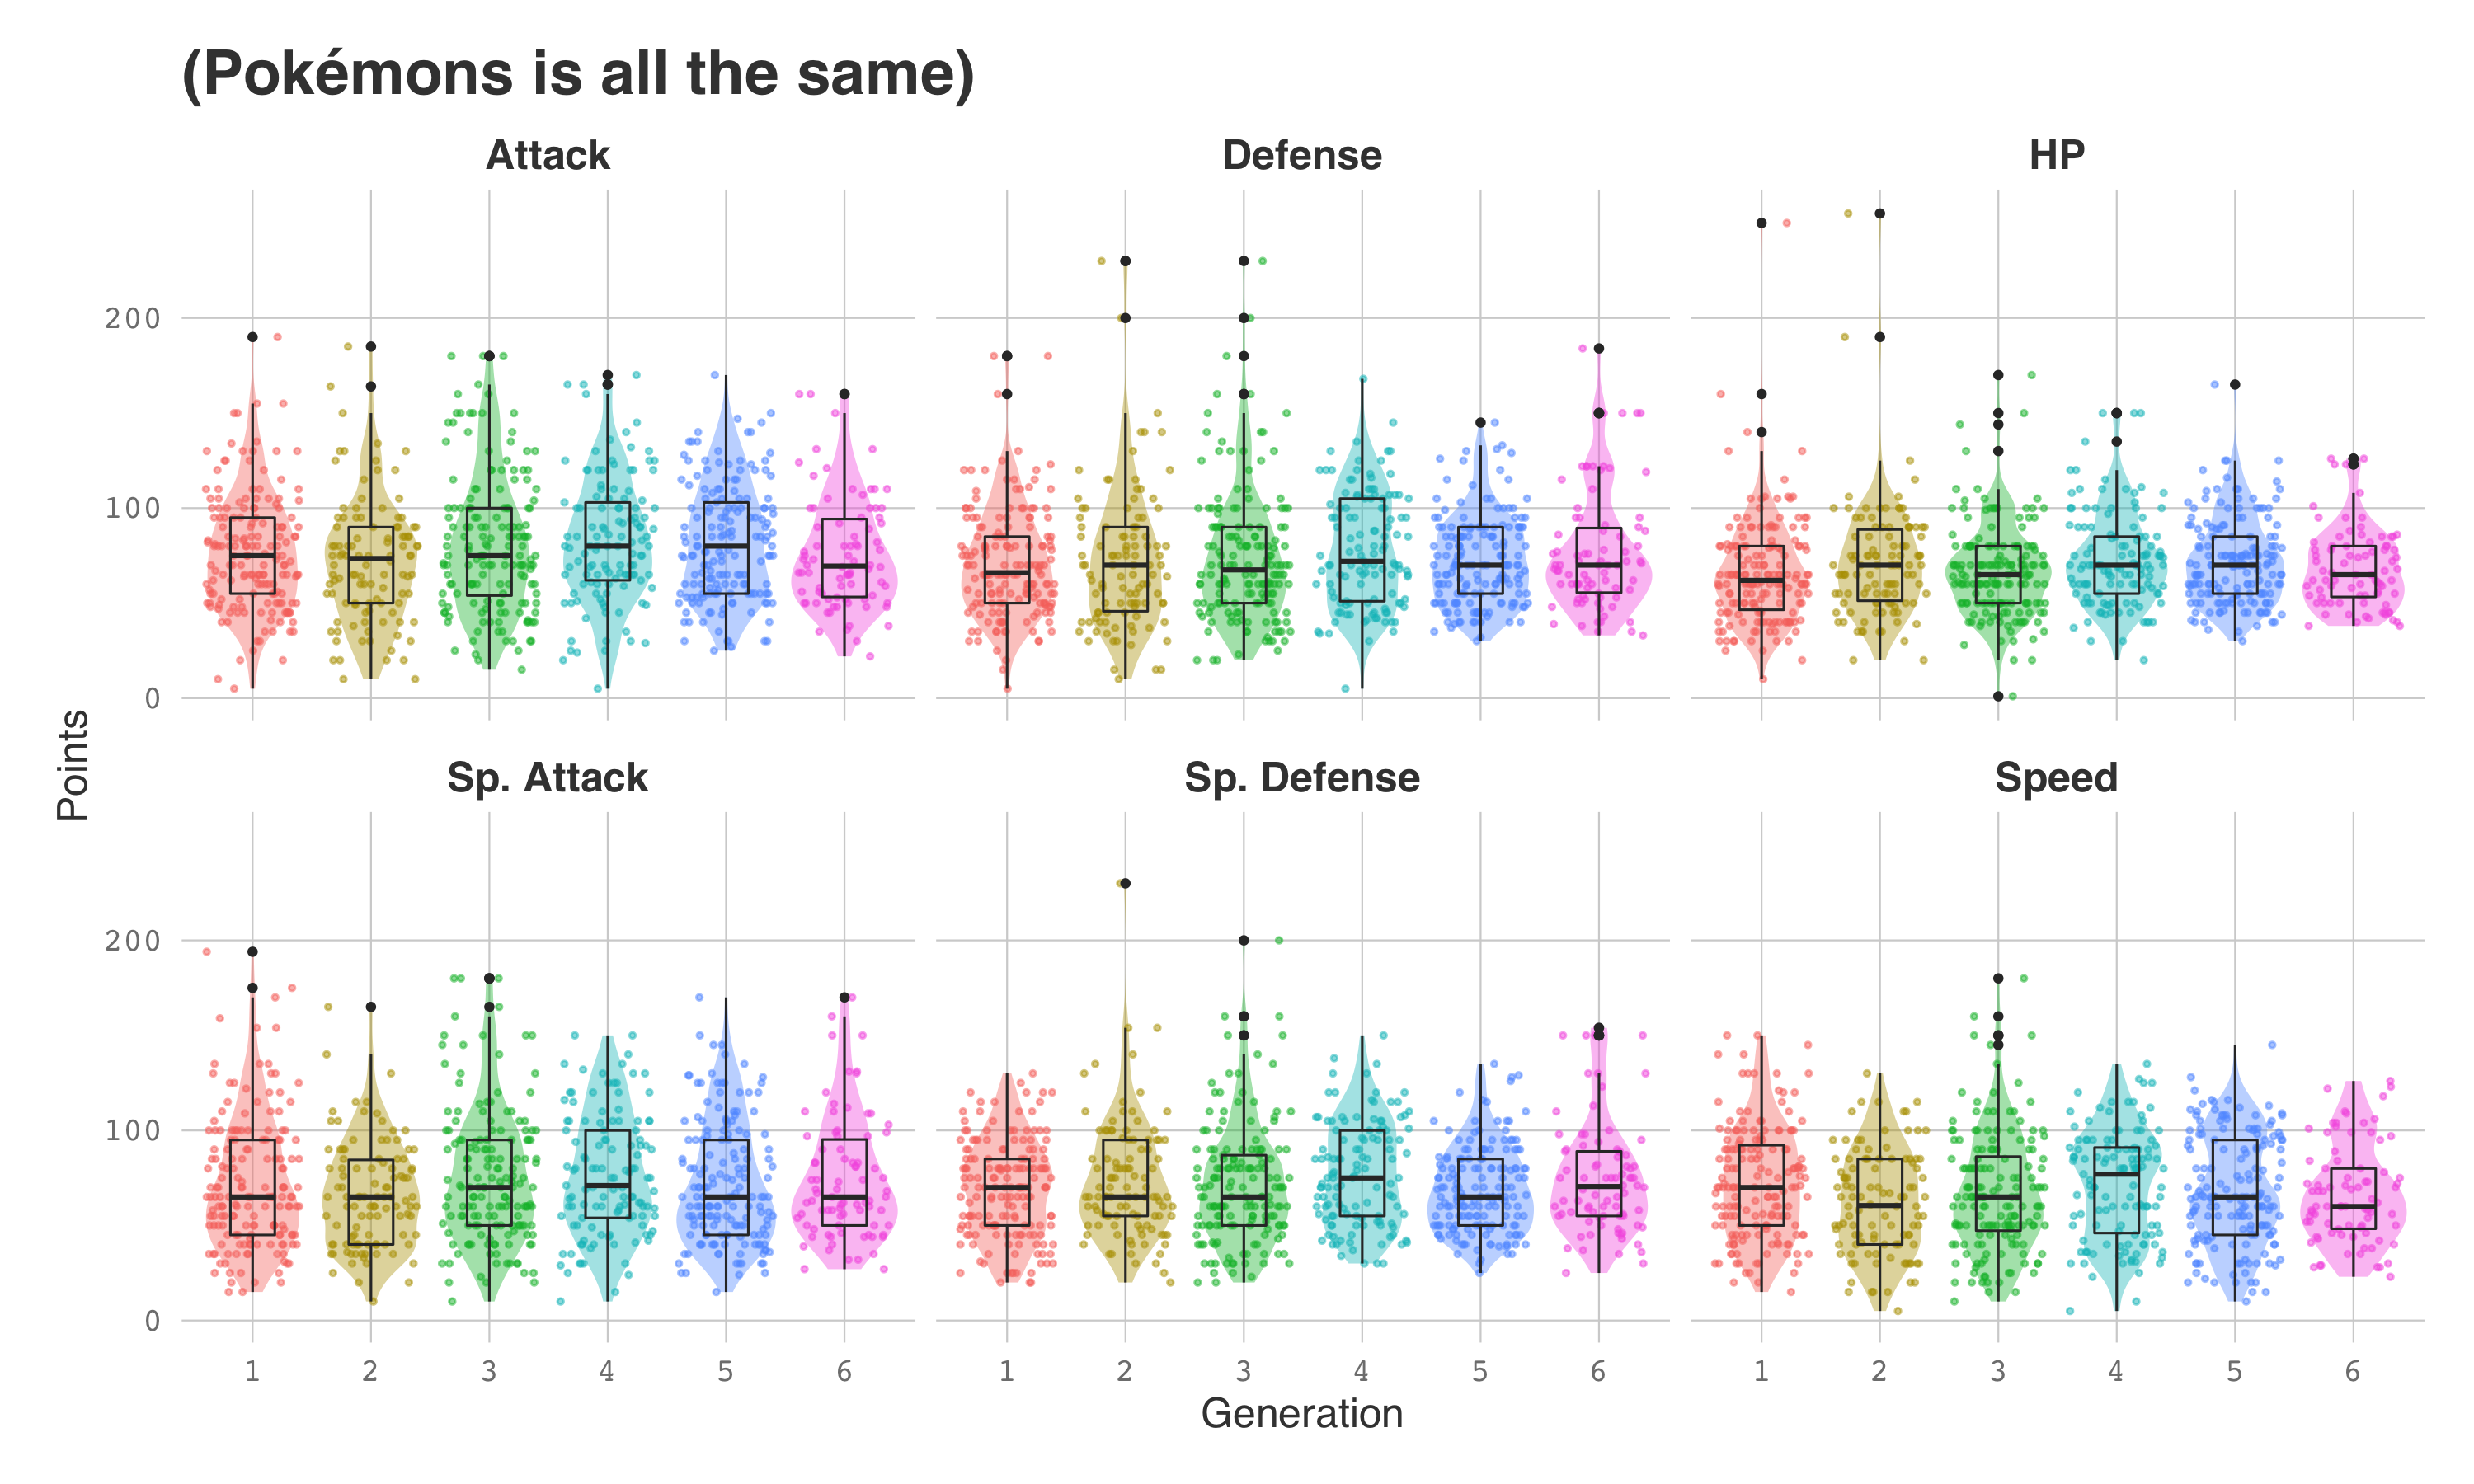
\includegraphics[width = \textwidth]{imgs/specs-gen-vio-box.png}
    \caption{Distribution of Pok\'emon Stats}
    \label{fig:poke-stats}
  \end{figure}


  A few other bits of syntax and notes:
  \begin{itemize}
    \item \verb+[ht]+ locates the float `here' on the page or on the top of the next page if there isn't enough space.  Alternately, can use \verb+[t!]+ (`top') or \verb+[b!]+ (`bottom'). The exclamation point overrides LaTeX's normal rules for placing figures.
    \item \verb+\caption+ inserts a caption.  Alternately, can use \verb+\caption*+ to inset an unnumbered caption.
    \item Several file formats will work, but in general, you should include ``vector'' graphics (such as \texttt{.pdf}s), since they are infinitely scalable without losing image detail. Stata and R can produce \texttt{.pdf} graphics with no problem at all.
  \end{itemize}



  You can also put multiple figures within the same command to get side-by-side figures, three across, a grid, etc. Include multiple \verb+\includegraphics+ commands and set the sizes appropriately to make it look how you want.\footnote{If you want a grid but don't want the figures to be large enough to force that to happen automatically, you can accomplish that using the tabular environment discussed below.} You could caption multiple figures in the same floating environment with the \texttt{subcaption} package.

  Labeling your figures and tables with the \verb+\label{labelname}+ command immediately after the caption allows you automatically to reference them later using \verb+Figure~\ref{labelname}+ (the tilde inserts a space that won't break across multiple lines). I could reference Figure~\ref{fig:poke-stats} using \verb+Figure~\ref{fig:poke-stats}+. The beauty of {\LaTeX} is that figure number is handled automatically, so you never have to re-number anything if you shuffle the order of figures.\footnote{Try doing that with Microsoft Word!}


\section{Tables}\label{tablessection}

  Tables are created using the \texttt{tabular} environment, generally within the \texttt{table} floating environment to allow for accessories (as with figures, this is good practice but not strictly necessary if you have no accessories).

  \newpage 
  This code produces the table below:
  \begin{verbatim}
\begin{table}[!ht]
\begin{center}
\caption{Selected Films}\label{film}
\begin{tabular}{l|c | c |  c | D{.}{.}{4}}
           & Acting & Writing   & Effects  & \multicolumn{1}{c}{Plot} \\ \hline
Inception  & good   & okay      & great    & 90.52   \\ \hline
The Artist & great  & none      & B\& W    & 100.0   \\ \hline
Birdemic   & bad    & atrocious & clip art & 3.1     \\ \hline
Twilight   & none   & none      & sparkly  & .111    \\
\end{tabular}
\end{center}
\end{table}
  \end{verbatim}

  \begin{table}[!ht]
  \begin{center}
  \caption{Selected Films}\label{film}
  \begin{tabular} {l|c | c |  c | D{.}{.}{4}}
           & Acting & Writing   & Effects  & \multicolumn{1}{c}{Plot} \\ \hline
Inception  & good   & okay      & great    & 90.52        \\ \hline
The Artist & great  & none      & B\& W    & 100.0         \\ \hline
Birdemic   & bad    & atrocious & clip art & 3.1     \\ \hline
Twilight   & none   & none      & sparkly  & .111    \\
  \end{tabular}
  \end{center}
  \end{table}

  What the syntax elements are doing:
  \begin{itemize}
  \item \verb+{l|c|c...}+ specifies the number of columns, their alignment (c=center, l=left, r=right), and vertical lines ( $|$ ) between them.
  %Note the difference between the lower case l- indicating left align, and the | symbol- indicating a vertical line and, typed with shift-backslash.
  \item \verb+D{.}{.}{4}+ aligns cells in that column on the decimal point (requires the \texttt{dcolumn} package).
  \item \verb+&+ specifies breaks between cells within the table.
  \item \verb+\\+ creates a line break at the end of each line of the table.
  \item \verb+\hline+ inserts a horizontal line.
  \item \verb+\caption+ inserts a caption, just like with figure
  \end{itemize}

  Additional notes:
  \begin{itemize}
  \item Most normal in-text style and mathematical commands (boldface, italics, equations, etc) work fine within tables.
  \item If a table needs to include a lot of information, and the font doesn't need to be huge to be readable, you can make the whole thing `small' or `footnotesize' to fit.
  \item Toggling `wrap' on/off in WinEDT will change the display settings with your code to see unbroken lines - very useful when editing wide tables or ones with lots of text modifying commands in the input that take up space. In TexShop, this can be toggled under `Source'-`Wrap Lines'
  \end{itemize}


  \begin{table}[!ht]
  \begin{center}
  \caption{Detective Comparison}\label{det}
  \begin{tabular} {l |c c | c c | c c |}
  \multicolumn{1}{c}{} & \multicolumn{2}{c}{L\&O: SVU} & \multicolumn{2}{c}{Literature}  & \multicolumn{2}{c}{Other} \\  \cline{2-7}
                    & Benson     & Stabler  & Holmes & Hardy Boys & Dick Tracy & Batman       \\ \cline{2-7}
  Loose Cannon    & 6       & 10         & 9      & 0        & 3     & 11             \\ \cline{2-7}
  Det. Ability           &  8   & 5     & 10    & 3          & 4      & 11           \\ \cline{2-7}
  Effectiveness   & 80\%  & 70\% & 95\% & 100\%      & 40\%     & 5\% \\ \cline{2-7}
  Tenure (yrs)  & 14+         & 12       & 23        & 1       & 66      & 75              \\ \cline{2-7}
  \end{tabular}
  \end{center}
  \end{table}

  Some new syntax introduced:
  \begin{itemize}
  \item \verb+\cline{2-7}+ inserts horizontal lines across columns 2 through 7.
  \item \verb+\multicolumn{2}{c}{text}+ merges adjacent cells to have a multiple-column cell, in this case spanning 2 columns and aligned in the center.
  \end{itemize}


  \begin{table}[!ht]
  \begin{center}
  \begin{footnotesize}
  \begin{tabular}{p{3.5in} r c r}
  Item                                                          & Unit Cost & Qty  &    Cost    \\ \hline
  \rule{0cm}{.5cm}\textit{Buying coffee to claim a table for the morning}       & \$3.00    &  60  &   \$150.00 \\
  \rule{0cm}{.5cm}\textit{Library books}                                        & \$0.00    & 45   &   \$0.00   \\
  \rule{0cm}{.5cm}\textit{Spinal realignment (needed after carrying library books up and down Bascom Hill)}   & \$150.00  & 1    &   \$150.00 \\
  \rule{0cm}{.5cm}\textit{Stress balls}                                         & \$4.50    & 3    &   \$13.50  \\
  \rule{0cm}{.5cm}\textit{Buying coffee to claim a table for the afternoon}        & \$3.00    & 60   &   \$150.00 \\
  \rule{0cm}{.5cm}\textit{Office supplies (pens, pencils, highlighters, tags, index cards, binders, cookies, ice cream)}& \multicolumn{2}{c}{(assorted)} & \$60.00 \\  
  \rule{0cm}{.5cm}\textit{Celebratory after-prelims steak (Tornado Room)}                                         & \$60.00    & 1    &   \$60.00  \\
  \rule{0cm}{.5cm} & \multicolumn{2}{r}{Total:} & \$642.50 \\ \hline
  \rule{0cm}{.5cm} & \multicolumn{2}{r}{Finishing Prelims:} & priceless \\ \cline{2-4}
  \end{tabular}
  \end{footnotesize}
  \end{center}
  \end{table}

  2 more handy new commands:
  \begin{itemize}

  \item \verb+p{3.5in}+ fixes the width of the column, allowing you to wrap text.
  \item \verb+\rule{0cm}{.5cm}+ creates a line with the specified width (here 0cm) and height (here .5cm).  This can be used to create an actual line or, as it is used here, to adjust the vertical spacing of cells (by making a line with 0 width, so it doesn't actually draw anything).
  \end{itemize}

  You can create sideways tables with the appropriately named \texttt{sidewaystable} package.

  \textbf{Some additional advice:} Minimize the extent to which you hand-create tables. R and Stata can generate {\LaTeX} code as output using the \texttt{stargazer}, \texttt{texreg}, \texttt{xtable} (for R), or \texttt{outtex} (for Stata) packages. Hand-typing tables introduces human error and makes your workflow less reproducible for anyone who wants to replicate your analysis, so relying on algorithms for creating tables is good practice.


\section{Arrays and Matrices}

  The tabular environment can also be used to draw arrays, matrices, and other similar objects using much of the same syntax as tables.  A few samples:
  \[
  B_1(q) = \left\{\begin{tabular}{l c l}
  0     & if & $q < \frac{1}{4}$ \\
  $[0,1]$   & if & $q = \frac{1}{4}$ \\
  1     & if & $q > \frac{1}{4}$ \\
  \end{tabular}\right.
  \]

  \[
  \textrm{Matrix} = \left[\begin{tabular}{cccc}
  1 & 0 & 0 & 0 \\
  0 & 1 & 0 & 0 \\
  0 & 0 & 1 & 0 \\
  0 & 0 & 0 & 1 \\
  \end{tabular}\right]
  \]

  \[
  \begin{bmatrix}
  4 & 5  \\
  2 & 0  \\
  1 & 7
  \end{bmatrix}
  \times
  \begin{bmatrix}
  8 & 4 & 0  \\
  6 & 3 & 4
  \end{bmatrix}
  =
  \begin{bmatrix}
  62 & 31 & 20  \\
  16 & 8  & 0  \\
  50 & 25 & 28 
  \end{bmatrix}
  \]

  \begin{itemize}
  \item \verb+\[+ and \verb+\]+ start and close the object.
  \item \verb+\left**+ and \verb+\right**+ define the boundaries of the object.  These can be curly brackets \verb+{+, parentheses \verb+(+, square brackets \verb+[+, or empty \verb+.+ (period).
  \item Matrix environments such as \texttt{bmatrix} provide similar functionality.
  \end{itemize}



\clearpage



\section{Good {\LaTeX} Practices}

  \begin{itemize}
    \item \textbf{Re-use code}. Copy and paste from old code you or someone else created, and modify as needed. No need to reinvent the wheel every time. Make a blank \texttt{.tex} file that has a preamble using your most-used external packages, keep it somewhere safe, and start all fresh papers with that template. %This code included.
    \item \textbf{Include comments}. Particularly as you're still learning, it's a good idea to write comments in your code to explain why you're doing things or how you're doing it.  It's also a nice way to include content that you're not sure if you'll use---put it in a comment and you still have it later if you want it back in.
    \item \textbf{Whenever you open something, close it immediately}. Whether you're beginning and ending environments or opening and closing parenthesis or brackets, always put the end in right away, then fill in the content in between. This will greatly cut down on syntax errors from forgetting to close things once you've gotten distracted by the substance. Some software will do this for you, so find handy software!
    \item \textbf{Compile early and often}. Bugs can be hard to find, so if you write a long document and it won't compile it is often frustrating and time-consuming to figure out where it's getting tripped up.  Compile often---anytime you do anything new or complicated---to make sure it's working; that way when errors occur you'll know where they are.
    \item \textbf{Debug in the order the errors appear.} When debugging a {\LaTeX}document, make sure that you start by fixing errors as early in the document as you can. Errors tend to cascade---failing to close an environment early in the document can result in multiple other problems later in the document. 
    \item \textbf{Comment-out lines to debug}. If you're getting errors and can't figure out why, try commenting-out complicated parts here and there to find the source that's tripping it up.
    \item \textbf{- $\neq$ -- $\neq$ ---}. Don't confuse your dashes, en dashes, and em dashes. You have a powerful typesetting system at your fingertips, make use of it! For those who can't remember when to use your en dash (--) and when to use your em dash (---), Wikipedia has your back (\url{http://en.wikipedia.org/wiki/Dash}).
  \end{itemize}


\section{Useful Resources}

\begin{itemize}
\item The Comprehensive \TeX~Archive Network (\url{http://www.ctan.org}).  In particular see the `Not So Short' guide at \url{http://ctan.tug.org/tex-archive/info/lshort/english/lshort.pdf} with tons of information on beginning and advanced topics.
\item The {\LaTeX} Wikibook (\url{https://en.wikibooks.org/wiki/LaTeX}). This is how I (Michael DeCrescenzo) learned {\LaTeX}.
\item {\TeX} Exchange (\url{http://tex.stackexchange.com/}). This site collects user questions related to working with {\LaTeX}. Other users offer answers and can ``upvote'' the best answers. The large user base results in very high quality answers to both common and obscure questions. Don't be afraid to post a question if you're unable to figure out a given issue. 
\item Crash Course in {\LaTeX} (\url{http://haptonstahl.org/latex/}). A very nice user-friendly website guide to {\LaTeX}, created by a Steve Haptonstahl, a (former) political methodologist.
\item Google (\url{https://www.google.com/}). If all else fails (or, perhaps, before searching through pages and pages of documentation) just search for what you're looking for --- there will be a user group discussion or a guide posted somewhere that explains how to do it.
\item Wikipedia's List of {\LaTeX} editors (\url{http://en.wikipedia.org/wiki/Comparison_of_TeX_editors}). There are various alternative {\LaTeX} editors that are of varying degrees of quality and price. Many are better than the default editors that come with various TeX distributions.  
\item Detexify (\url{http://detexify.kirelabs.org}). Need to include a symbol but don't know what it's called or how to enter it into LaTex? Draw the symbol using this tool, and the program will return the command to draw it. For example, draw that ``trident-looking thing'' and the tool will tell you how to make a $\psi$.
\item Overleaf (\url{https://www.overleaf.com/}). Cloud-based {\LaTeX} editor which allows documents to be edited by multiple individuals at the same time and which compiles in real-time. 
\end{itemize}

\end{document}